%% We use `subfiles' package
\documentclass[preamble.tex]{subfiles}
\begin{document}

\clearpage

\chapter{Considerations for fusing lockstep consumers}
\label{ch:zipping-problems}

This appendix follows from the discussion of @zipWith@$N$ combinators in Section~\ref{sec:zipping} on page~\pageref{sec:zipping}.

In general the fusion of combinators that consume multiple arrays in lockstep (@zipWith@$N$ family of combinators, @indices_s@, @replicate_s@, etc..) faces the following two problems:

\begin{enumerate}
\item The lengths of the input arrays may be different.
\item The loops producing some of all of the input arrays may not produce elements in every iteration.
\end{enumerate}

The following two sections discuss the two problems in turn and offer potential solutions. It should be noted that neither of the problems are affecting the fusion of \name{Data Parallel Haskell} programs and can be left as future work.


\clearpage
\section{Inputs of different lengths}

In the standard \Haskell library the result list of @zipWith@ combinator has the same length as the shortest of its inputs. In the \Loop language this could easily be expressed by setting the output length to be the minimum of the input array lengths and adjusting the iteration range appropriately:

\begin{loopcode}[%
  literate=
    {_1}{{\sub{zip}}}2
    {_2}{{\sub{xs}}}1
    {_3}{{\sub{ys}}}1,
]
init_1/_2/_3:
  let len_1 = min len_2 len_3

guard_1/_2/_3:
  unless ix_1 < len_1 | done_1
\end{loopcode}

However, there are still implications of this approach. Consider the program in Figure~\ref{fig:zipProblem1}. The @ys@ array is consumed both by @zipWith@ and @map@. Supposing that @xs@ is shorter than @ys@ it makes it harder (though not impossible) to compute both @xys@ and @zs@ in the same loop.

\begin{figure}

\begin{subfigure}{.6\textwidth}
\begin{hscode}
let xys = zipWith (*) xs ys
    zs  = map (+1) ys
in  (xys, zs)
\end{hscode}
\end{subfigure}%
%
\begin{subfigure}[right]{.4\textwidth}
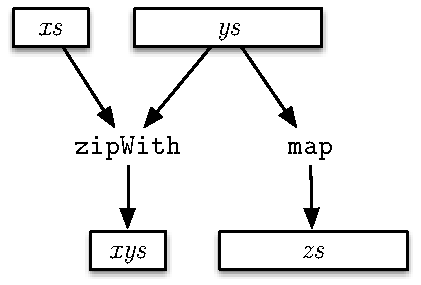
\includegraphics[center,scale=\omniscale]{img/DFD-zipWithMap}
\end{subfigure}

\caption{Zipping arrays of different lengths. \Haskell code (left) and the corresponding data flow diagram (right).}
\label{fig:zipProblem1}
\end{figure}

In order to successfully fuse the above example the \Loop language needs to be able to express overlapping loop ranges. In this particular example a portion of the index range should be processed by both @zipWith@ and @map@ operations, and the rest with just the @map@.

Since \LiveFusion was designed to target \DPH\idph, and \DPH statically guarantees the inputs to be of the same lengths, the restriction on accepted input lengths is justified.



\clearpage
\section{Skipping elements in the inputs}

\LiveFusion has support for fusing loops which do not produce an elements in every iteration. The most prominent of those is perhaps the @filter@ combinator. If the combinator pipeline producing an input to @zipWith@ contains a @filter@, fusing them becomes more challenging.

Consider the following example:

\begin{hscode}
let xs = filter odd [0..9]
    ys = [11..15]
    zs = zipWith (*) xs ys
in  zs
\end{hscode}

While @zipWith@ is supposed to consume elements from @xs@ and @ys@ in a lockstep, producing both those elements will not always happen in the same iteration. @ys@ array does not pose a problem, it is guaranteed to produce one element in each iteration. However, the addition of @filter@ into the equation for @xs@ will mean that the loop for @xs@ may require more than one iteration to produce an element. If the @filter@ skips an element the loop for @ys@ must wait.


\subsection{A solution}

Considering a potential implementation of the same program in a procedural language reveals that it is still possible to only use one overall loop for computing @zs@.

However, a separate nested loop is required for computing the elements of @xs@. This loop will exit when the @filter@ predicate is satisfied.


\begin{figure}[ht]

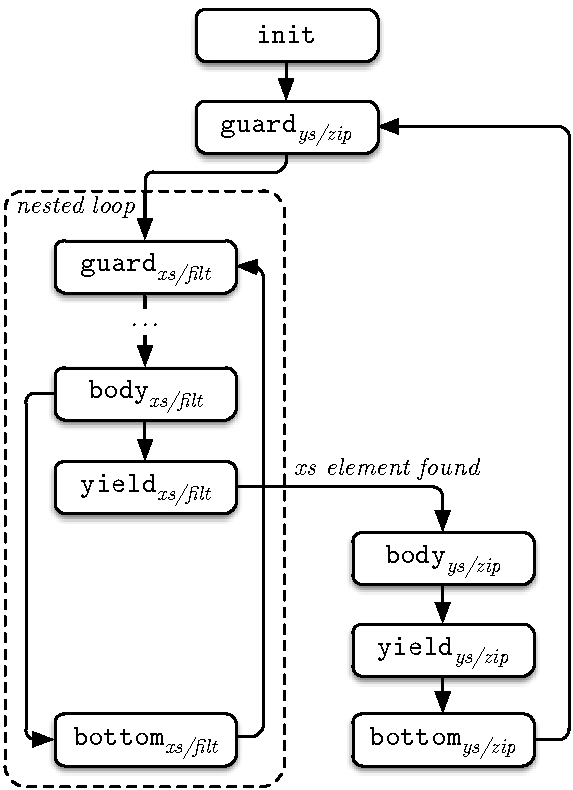
\includegraphics[center,scale=\omniscale]{img/CFG-ZipFilter}

\caption{\Loop language CFG for a nested loop solution to lockstep consumption of producers that may skip.}
\label{fig:CFG-zipWithFilter}
\end{figure}


Figure~\ref{fig:CFG-zipWithFilter} presents a potential solution to the problem expressed as a control flow graph in the \Loop language. The bodies of @zipWith@ and @ys@ are merged together in the outer loop while the whole of @xs@ including @filter@ is an loop which is entered before the body of @zipWith@ is executed.


\subsection{Implications}

A solution described above is plausible in \LiveFusion. However, it requires more sophisticated analysis of the combinator graph.

Again, the \DPH system which is the primary target of \LiveFusion is guaranteed to feed @zipWith@ combinator with uniformly produced arrays. Even if the input arrays are filtered they all skip of produce an element at the same time.


\end{document}